%--------------------
% Packages
% -------------------
\documentclass[11pt,english]{article}
\usepackage{amsfonts}
\usepackage[left=2.5cm,top=2cm,right=2.5cm,bottom=3cm,bindingoffset=0cm]{geometry}
\usepackage{amsmath, amsthm, amssymb}
\usepackage{tikz}
\usetikzlibrary{calc}
\usetikzlibrary{decorations.pathreplacing,calligraphy}
\usepackage{fancyhdr}
%\usepackage{currfile}
\usepackage{nicefrac}
\usepackage{cite}
\usepackage{graphicx}
\usepackage{caption}
\usepackage{longtable}
\usepackage{rotating}
\usepackage{lscape}
\usepackage{booktabs}
\usepackage{float}
\usepackage{placeins}
\usepackage{setspace}
\usepackage[font=itshape]{quoting}
\onehalfspacing
\usepackage{mathrsfs}
\usepackage{tcolorbox}
\usepackage{xcolor}
\usepackage{subcaption}
\usepackage{float}
\usepackage[multiple]{footmisc}
\usepackage[T1]{fontenc}
\usepackage[sc]{mathpazo}
\usepackage{listings}
\usepackage{longtable}
\definecolor{cmured}{RGB}{175,30,45}
\definecolor{macroblue}{RGB}{56,108,176}
\usepackage[format=plain,
            labelfont=bf,
            textfont=]{caption}
\usepackage[colorlinks=true,citecolor=macroblue,linkcolor=macroblue,urlcolor=macroblue]{hyperref}
\usepackage{varioref}
\usepackage{chngcntr}
\usepackage{datetime}

\definecolor{darkgreen}{RGB}{30,175,88}
\definecolor{darkblue}{RGB}{30,118,175}
\definecolor{maroon}{rgb}{0.66,0,0}
\definecolor{darkgreen}{rgb}{0,0.69,0}

%Counters
\newtheorem{theorem}{Theorem}[section] 
\newtheorem{proposition}{Proposition}
\newtheorem{lemma}{Lemma}
\newtheorem{corollary}{Corollary}
\newtheorem{assumption}{Assumption}
\newtheorem{axiom}{Axiom}
\newtheorem{case}{Case}
\newtheorem{claim}{Claim}
\newtheorem{condition}{Condition}
\newtheorem{definition}{Definition}
\newtheorem{example}{Example}
\newtheorem{notation}{Notation}
\newtheorem{remark}{Remark}


\hypersetup{ 	
pdfsubject = {},
pdftitle = {TidyTuesday Week 34},
pdfauthor = {Pranay Gundam},
linkcolor= macroblue
}


\title{\textbf{TidyTuesday Week 34}}
\author{Pranay Gundam}


%-----------------------
% Begin document
%-----------------------
\begin{document}

\maketitle

\tableofcontents

\section{Weekly Summary}


\section{Date: 2024-08-20}
\noindent \textbf{Series ID: CIU2030000300000I} 

\noindent This series is titled Employment Cost Index: Total benefits for Private industry workers in Service occupations and has a frequency of Quarterly. The units are Index Dec 2005=100 and the seasonal adjustment is Not Seasonally Adjusted.The observation start date is 2001-01-01 and the observation end date is 2024-04-01.The popularity of this series is 1. \\ 

\noindent \textbf{Series ID: CUURA100SAT1} 

\noindent This series is titled Consumer Price Index for All Urban Consumers: Private Transportation in Northeast - Size Class A and has a frequency of Monthly. The units are Index 1982-1984=100 and the seasonal adjustment is Not Seasonally Adjusted.The observation start date is 1977-12-01 and the observation end date is 2024-08-01.The popularity of this series is 1. \\ 

\subsection{Regression Table}
\begin{center}
\begin{tabular}{lclc}
\toprule
\textbf{Dep. Variable:}        & value\_fred\_THREEFF4 & \textbf{  R-squared:         } &     0.941   \\
\textbf{Model:}                &          OLS          & \textbf{  Adj. R-squared:    } &     0.941   \\
\textbf{Method:}               &     Least Squares     & \textbf{  F-statistic:       } & 1.366e+05   \\
\textbf{Date:}                 &    Tue, 20 Aug 2024   & \textbf{  Prob (F-statistic):} &     0.00    \\
\textbf{Time:}                 &        07:35:04       & \textbf{  Log-Likelihood:    } &   -6380.6   \\
\textbf{No. Observations:}     &           8639        & \textbf{  AIC:               } & 1.277e+04   \\
\textbf{Df Residuals:}         &           8637        & \textbf{  BIC:               } & 1.278e+04   \\
\textbf{Df Model:}             &              1        & \textbf{                     } &             \\
\textbf{Covariance Type:}      &       nonrobust       & \textbf{                     } &             \\
\bottomrule
\end{tabular}
\begin{tabular}{lcccccc}
                               & \textbf{coef} & \textbf{std err} & \textbf{t} & \textbf{P$> |$t$|$} & \textbf{[0.025} & \textbf{0.975]}  \\
\midrule
\textbf{const}                 &      -1.3247  &        0.016     &   -82.497  &         0.000        &       -1.356    &       -1.293     \\
\textbf{value\_fred\_THREEFF9} &       1.0370  &        0.003     &   369.572  &         0.000        &        1.031    &        1.042     \\
\bottomrule
\end{tabular}
\begin{tabular}{lclc}
\textbf{Omnibus:}       & 1515.440 & \textbf{  Durbin-Watson:     } &    0.001  \\
\textbf{Prob(Omnibus):} &   0.000  & \textbf{  Jarque-Bera (JB):  } &  424.089  \\
\textbf{Skew:}          &  -0.275  & \textbf{  Prob(JB):          } & 8.13e-93  \\
\textbf{Kurtosis:}      &   2.064  & \textbf{  Cond. No.          } &     17.3  \\
\bottomrule
\end{tabular}
%\caption{OLS Regression Results}
\end{center}

Notes: \newline
 [1] Standard Errors assume that the covariance matrix of the errors is correctly specified.

\subsection{Regression Plot}
\begin{figure}
\centering
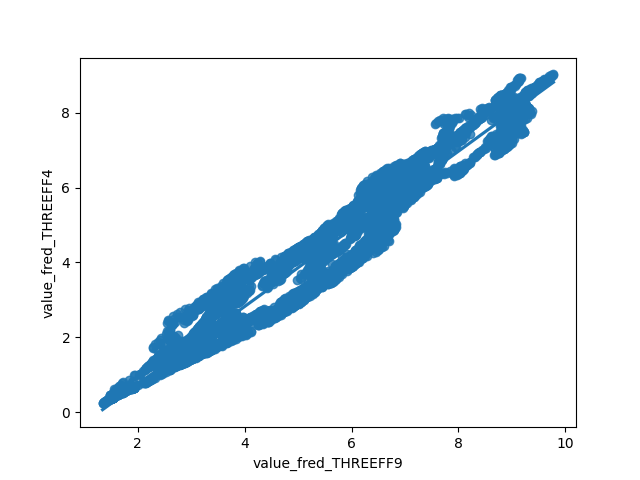
\includegraphics[scale = 0.9]{plots/plot_2024-08-20.png}
\caption{Regression Plot for 2024-08-20}
\end{figure}
\newpage

\include{tex_things/day_2024-08-21}
\include{tex_things/day_2024-08-22}
\include{tex_things/day_2024-08-23}
\include{tex_things/day_2024-08-24}
\include{tex_things/day_2024-08-25}
\include{tex_things/day_2024-08-26}

\end{document}
